%
% geometry.tex -- L"osung linearer Differentialgleichungen
%
% (c) 2016 Prof Dr Andreas Mueller, Hochschule Rapperswil
%
\chapter{Geometrische Eigenschaften\label{chapter:geometrie}}
\lhead{}
\rhead{Geometrische Eigenschaften}
Die Geometrie schr"ankt die m"oglichen Bahnen eines
Differentialgleichungssystems bereits wesentlich ein.
In einem eindimensionalen autonomen System sind keine
Schwingungen m"oglich, in einem zweidimensionalen
System gibt es keine chaotischen Bewegungen.
Ziel dieses Kapitels ist, in diese geometrische
Denkweise einzuf"uhren.
Das Buch \cite{skript:hirsch} f"uhrt diesen Ansatz weiter bis zu
einer Einf"uhrung in chaotische Bewegung.

\section{Autonome Systeme}
\begin{figure}
\centering
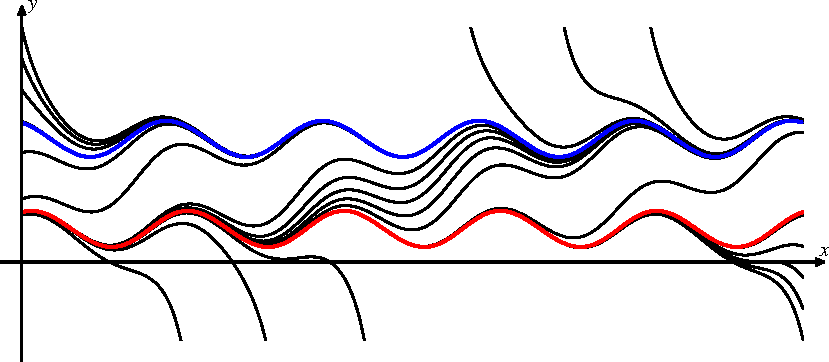
\includegraphics{chapters/images/geometrie-13.pdf}
\caption{Entwicklung des Systems~(\ref{geometrie:harvest-equation})
mit $a=5$ und $h=0.8$
\label{geometrie:harvest-graph}}
\end{figure}%
Ein eindimensionales System k"onnen wir schreiben als
\[
y'=f(x,y).
\]
Die L"osungskurven dieses Systems k"onnen wir in einem $x$-$y$-Diagramm
als Graphen darstellen.
Zum Beispiel k"onnen wir die Entwicklung des Systems
\begin{equation}
y' = ay(1-y)-h(1+\sin 2\pi x)
\label{geometrie:harvest-equation}
\end{equation}
wie in Abbildung~\ref{geometrie:harvest-graph} darstellen.
Dieses nicht-autonome System hat zwei Grenzzyklen: 
Anfangswerte oberhalb der roten Kurve f"uhren zu L"osungskurven, die
sich f"ur zunehmendes $x$ der blauen Kurve ann"ahern.
Anfangswerte unterhalb der blauen Kurve f"uhren zu L"osungskurven, die
sich f"ur abnehmendes $x$ der roten Kurve n"ahern.

Startwerte in der N"ahe der roten Kurve sind nicht stabil,
die Entwicklung f"ur zunehmende $x$ f"uhrt den Wert immer weiter von
der roten Kurve weg.
Lag der Startwert unterhalb der roten Kurve, wird die L"osung gegen
$-\infty$ divergieren.
Alle anderen L"osungen konvergieren gegen die blaue Kurve.

Offenbar ist es ziemlich schwierig, das
System~(\ref{geometrie:harvest-equation}) "uber gr"ossere $x$-Intervalle
zu verstehen. 
Zum Beispiel h"angt das Verhalten davon ab, ob der Startwert zwischen den
farbigen Kurven liegt oder ausserhalb, und diese h"angt vom Start-$x$ ab.

In Kapitel~\ref{chapter:grundlagen} wurde beschrieben, wie jedes
Differentialgleichungssystem, m"oglicherweise nach Erweiterung um eine
explizite Zeitkoordinate, zu einem autonomen System gemacht und damit
durch ein Vektorfeld ersetzt werden kann,
und wie die L"osungen als Bahnen eines Teilchens in einem zeitlich
unver"anderlichen Vektorfelde verstanden werden k"onnen.
Daraus ergibt sich auch, dass das Verhalten der L"osungen einer
Differentialgleichungen studiert werden kann, ohne dass man
die Abh"angigkeit von $x$ im Detail kennt.
Die Bahnen zerlegen den Raum und k"onnen sich nicht schneiden,
so schr"ankt die Geometrie des Raumes die M"oglichkeiten f"ur das
Verhalten der L"osung "uber lange Zeiten ein.
Besonders ausgepr"agt sind diese Einschr"ankungen im zweidimensionalen
Raum.
Eine geschlossene Kurve in der Ebene unterteilt diese in zwei Bereiche,
keine L"osung kann vom einen Bereich in den anderen f"uhren.

Ein Parameter in der Differentialgleichung modifiziert das Vektorfeld,
und kann damit Eigenschaften von L"osungen "uber lange Zeiten ver"andern.
Zum Beispiel k"onnen periodische Bahnen sich aufl"osen und zu Spiralbahnen
werden.

Wir gehen in diesem Kapitel immer von einem autonomen System
\[
\frac{d}{dx}y(x)=f(y),
\]
wobei das Vektorfeld $f(y)$ nicht von $x$ abh"angt.
Uns interessieren die geometrische Eigenschaften der L"osungskurven, 
soweit sie sich direkt aus den Eigenschaften des Vektorfeldes ableiten
lassen.
Insbesondere interessieren uns also spezielle Punkte des Vektorfeldes,
zum Beispiel Nullstellen.


%
% Spezielle Punkte und Bahnen
%
\section{Spezielle Punkte und Bahnen}
Das Verhalten der L"osungskurven "uber lange Zeiten wird wesentlich
beeinflusst von Punkte, wo der Punkt auf der Bahn anh"alt oder sogar
die Richtung umkehrt, und von Punkten, in die ein Punkt periodisch
zur"uckkommt.

%
% Kritische Punkte
%
\subsection{Kritische Punkte}
Wir betrachten zun"achst einen Punkt $y_0$ in dem $f(y_0)\ne 0$.
Dann gilt $f(y)\ne 0$ auch f"ur Punkte $y$, die gen"ugend nahe an 
$y_0$ sind.
Eine L"osungskurve durch $y_0$ hat im Punkt $y_0$ die Tangentenrichtung
$f(y_0)$.
In einer gen"ugend kleinen Umgebung von $y_0$ werden sich verschiedene
L"osungskurven nicht schneiden.
Ein solcher Schnittpunkt w"are ein Anfangsbedingung f"ur zwei
verschiedene L"osungen, aber der Eindeutigkeitssatz f"ur die
L"osung einer Differentialgleichung sagt, dass es zu jeder 
Anfangsbedingung nur eine L"osung geben kann.
Dies bedeutet, dass in einer Umgebung des Punktes $y_0$ nichts
spannendes passiert, die Bahnen sehen ungef"ahr aus wie in
Abbildung~\ref{geometrie:parallelebahnen}.
\begin{figure}
\centering
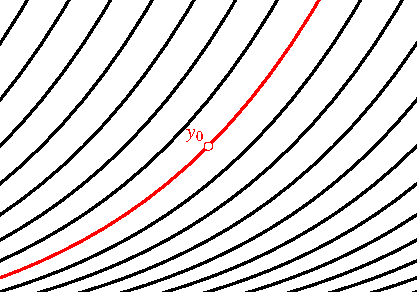
\includegraphics{chapters/images/geometrie-12.pdf}
\caption{Verlauf der Bahnen eines autonomen Differentialgleichungssystems
in der N"ahe eines Punktes $y_0$ mit $f(y_0)\ne 0$.
\label{geometrie:parallelebahnen}}
\end{figure}

Von besonderem Interesse sind daher Punkte, an denen das Vektorfeld
verschwindet:

\begin{definition}
$y$ heisst {\em kritischer Punkt} des Vektorfeldes $f$, wenn $f(y)=0$.
\end{definition}

Dass in einem kritischen Punkt das Vektorfeld verschwindet bedeutet nicht,
dass die Bahn nicht dar"uber hinweg fortgesetzt werden kann,
wie das folgende Beispiel zeigt.

\begin{beispiel}
Das eindimensionale Gleichungssystem
\[
y'=\sqrt{|y|}
\]
hat einen kritischen Punkt bei $y=0$.
Die Funktion
\begin{equation}
y(x)=\frac14x^2\operatorname{sign}(x)
\label{geometrie:1dimkritloesung}
\end{equation}
ist eine L"osungsfunktion, denn
\begin{align*}
y'(x)&=\frac12|x|\\
\sqrt{\left|\frac14x^2\operatorname{sign}(x)\right|}
&=
\sqrt{\frac14x^2}
=
\frac12|x|=y'(x).
\end{align*}
Trotzdem erreicht $y(x)$ jeden beliebigen Punkt der $y$-Achse, denn 
\[
x=2\sqrt{|y|}\operatorname{sign}(y)
\]
ist die Umkehrfunktion von $y(x)$. 
Die L"osungskurve bewegt sich also "uber den kritischen Punkt hinweg.
\begin{figure}
\centering
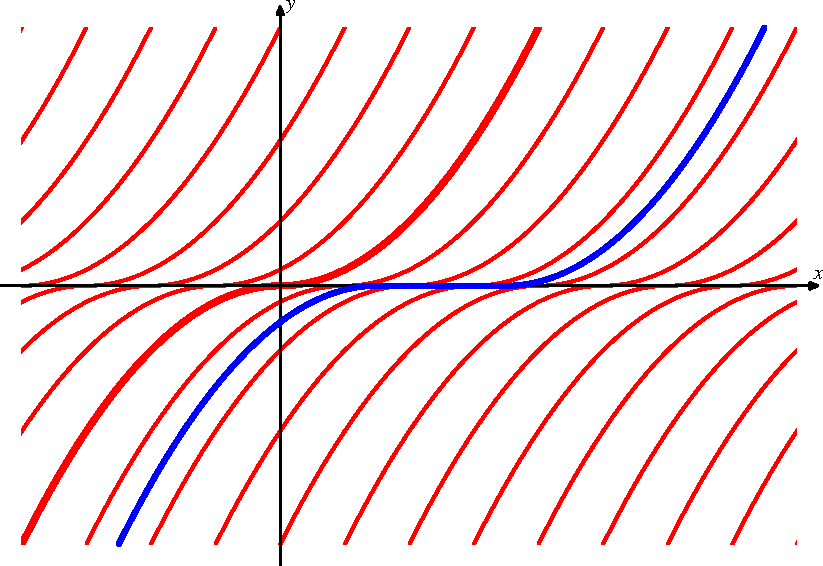
\includegraphics{chapters/images/geometrie-1.pdf}
\caption{Bahnen das Differentialgleichungssystems $y'=\sqrt{|y|}$
k"onnen den kritischen Punkt bei $y=0$ traversieren.
Die L"osung~(\ref{geometrie:1dimkritloesung}) ist etwas fetter rot
eingezeichnet.
L"osungen k"onnen aber auch beliebig lange im Punkt $y$ verweilen,
wie die blaue Kurve illustriert.
\label{geometrie:1dimkrit}}
\end{figure}
Abbildung~\ref{geometrie:1dimkrit} zeigt die Bahnen.
Die L"osung~(\ref{geometrie:1dimkritloesung}) ist nicht die einzige.
Andere L"osungen bestehen jeweils aus einem Ast der Kurve mit positiven
$y$ und einem mit negativen $y$, dazwischen kann die L"osung beliebig lange
im kritischen Punkt verweilen.
F"ur den Punkt $y=0$ ist also der Eindeutigkeitssatz verletzt, zur
Anfangsbedingung $y=0$ gibt es beliebig viele L"osungen.
\end{beispiel}

%
% Linearisierung
%
\subsection{Linearisierung}
In einem kritischen Punkt $y_0$ verschwinden alle Komponenten von $f(y_0)$.
Falls $f$ stetig differenzierbar ist, k"onnen wird $f$ in einer Umgebung
des kritischen Punktes in erster Ordnung approximieren:
\[
f(y)=\frac{\partial f}{\partial y}(y-y_0) + o(|y-y_0|)
\]
Die partielle Ableitung, die Jacobi-Matrix, ist eine $n\times n$-Matrix.
In einer Umgebung eines kritischen Punktes ist die Gestalt der Bahnen also
im wesentlichen durch die Jacobi-Matrix bestimmt.

\begin{beispiel}
Wir betrachten als Beispiel die eindimensionale ($n=1$) Differentialgleichung
\[
y'=f(y)=y,
\]
die in $y_0=0$ einen kritischen Punkt hat.
Die Jacobi-Matrix ist konstant: $f'(y)=1$.
L"osungskurven mit Anfangsbedingungen $>0$ werden daher anwachsen,
w"ahrend L"osungskurven mit Anfangsbedingungen $<0$ abnehmen werden.
Die L"osungskurven werden daher vom kritischen Punkt ``abgestossen''.

W"ahlen wir stattdessen das System
\[
y'=f(y)=-y,
\]
dann ist die Jacobi-Matrix $f'(y)=-1$, und wir k"onnen analog schliessen,
dass L"osungskurven immer zum kritischen Punkt hinstreben.
\end{beispiel}

\begin{beispiel}
Das Beispiel im letzten Abschnitt verwendet
\[
y'=f(y)=\sqrt{|y|}
\]
ist im kritischen Punkt $y=0$ nicht stetig differenzierbar, daher ist
eine lineare Approximation nicht m"oglich.
Das fr"uher beobachtete Verhalten, dass sich L"osungskurven auf der
einen Seite vom kritischen Punkt entfernen, auf der anderen aber ann"ahern,
kann nur auftreten, wenn auch $f'(0)=0$ gilt, so dass wir $f$ in zweiter
Ordnung als
\[
y'=f(y)=\frac12 f''(0)y^2.
\]
Diese Differentialgleichung hat die Funktion
\[
y(x)=-\frac{2}{f''(0)x+C}
\]
als L"osung.
Je nach Wert von $C$ bekommen wir eine L"osung, f"ur $x>0$ anwachsen
oder abfallen, wenigstens f"ur ein kleines Intervall.
Die L"osung n"ahert sich dem kritischen Punkt, oder entfernt sich, je
nachdem auf welcher Seite die L"osungskurve beginnt.
\end{beispiel}

%
% Eindimensionale Systeme
%
\section{Eindimensionale Systeme}
Wir untersuchen in diesem Abschnitt das Verhalten eindimensionaler autonomer
Systeme.
Ein solches System hat die Form
\[
y'=f(y),
\]
und kann sofort mit Hilfe von Separation der Variablen gel"ost werden:
\[
\int\frac{dy}{f(y)} = t+C,
\]
was nat"urlich nur funktioniert, wenn $f$ konstantes Vorzeichen hat.
Daraus folgt, dass ein Startwert $y_0$, f"ur den $f(y_0)>0$ ist,
zu einer monoton wachsenden L"osung f"uhrt, w"ahrend $f(y_0)<0$
bedeutet, dass die L"osung monoton f"allt.
Erf"ullt ein Startwert $f(y_0)=0$, dann ist $y(x)=y_0$ eine
L"osung der Differentialgleichung.
Die kritischen Punkte von $f$ strukturieren also wie erwartet die
L"osungsmenge.
Wir suchen eine "ubersichtliche Visualisierung dieser Beobachtung
und wollen verstehen, wie sich die Struktur in Abh"angigkeit
von einem Parameter in der Differentialgleichung ver"andern kann.

%
% Mögliche Phasendiagramme in einer Dimension
%
\subsection{Phasenportraits}
Seien jetzt $y_1,y_2,\dots$ Nullstellen der Funktion $f(y)$.
Dann sind die Funktion $y(x)=y_i$ L"osungen der Differentialgleichung
$y'=f(y)$.
Die Bewegung zwischen den Nullstellen wird vollst"andig dominiert durch
das Vorzeichen von $f(y)$ zwischen den Nullstellen.
Wir k"onnen dies in einem sogenannten Phasen-Portrait visualisieren.
Abbildung~\ref{geometrie:phasenportrait} zeigt die L"osungen der
Differentialgleichung
\begin{equation}
y'=f(y)=y^3-y
\label{geometrie:cube}
\end{equation}
Die Nullstellen dieser Funktion sind $-1$, $0$ und $1$.
\begin{figure}
\centering
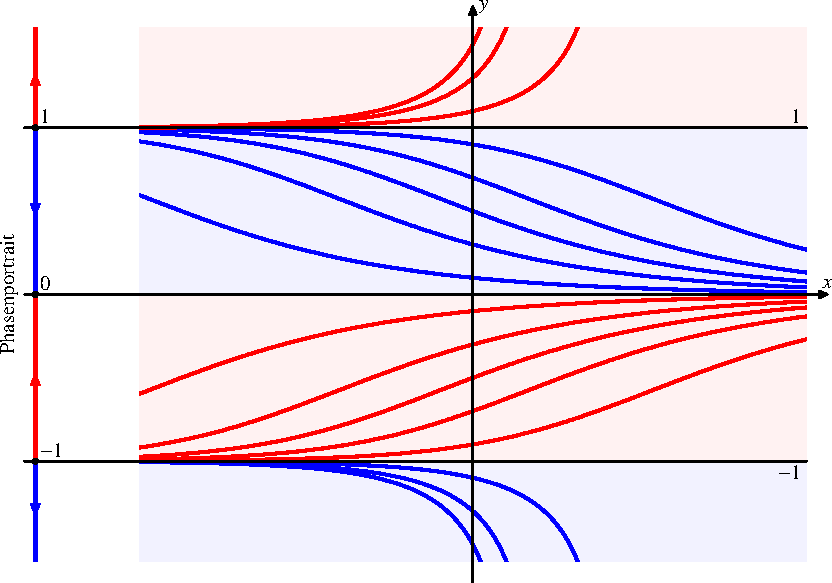
\includegraphics{chapters/images/geometrie-14.pdf}
\caption{Fluss der Differentialgleichung~(\ref{geometrie:cube}) und
Phasenportrait
\label{geometrie:phasenportrait}}
\end{figure}
Die exakte Abh"angigkeit von $x$ ist oft nicht wichtig, entscheidend
ist nur die Tatsache, dass Punkte im blauen Gebiet sich mit zunehmendem
$x$ nach unten bewegen, w"ahrend Punkte im roten Gebiet sich nach
oben bewegen.
Diese Information wird auch durch das Phasenportrait am linken
Rand der Abbildung~\ref{geometrie:phasenportrait} dargestellt.
Der Vortail eines Phasenportraits gegen"uber der Darstellung
der L"osung ist, dass sie mit einer Dimension auskommt.

%
% Mögliche Änderungen (Bifurkationen) der Phasendiagramme
%
\subsection{Bifurkationen\label{geometrie:subsection:bifurkationen}}
Betrachten wir jetzt eine Differentialgleichung, die ausserdem von einem
Parameter $b$ abh"angt:
\[
y'=f(y,b).
\]
Das Phasenportrait wird sich ver"andern, wenn $b$ variert, wir
m"ochten die verschiedenen dabei m"oglichen "Uberg"ange verstehen
k"onnen.
Es interessiert vor allem kleine "Anderungen in der Umgebung eines
Wertes $b_0$.
Dabei kommt es vor allem darauf an, dass mit Nullstellen passiert, und
welches Vorzeichen $f$ links und rechts von der Nullstelle hat.
Wir gehen daher davon aus, dass $f$ f"ur $b_0$ an der Stelle $y=0$
hat, dass also $a_0(b_0)=0$ ist.

Wenn $a_1(b_0)\ne0$ ist, also wenn $f'(0, b_0)\ne 0$ ist, dann 
gilt dies auch in einer Umgebung von $b_0$, und daher wird die
Nullstelle in erster N"aherung nur verschoben:
\[
y_0(b) \simeq -\frac{f(0,b)}{f'(0,b)},
\]
Das Phasenportrait erlebt also keine grundds"atzlichen "Anderung.

\subsubsection{Sattel-Knoten-Bifurkation}
Wir betrachten jetzt den Fall $f(0,b_0)=0$ und $f'(0,b_0)=0$, die Funktion
$f$ ist f"ur $b=b_0$ quadratisch, mit einer Nullstelle im Scheitel.
Variert $b$, wird zwar der Graph von $y\mapsto f(y,b)$ seine
Gestalt "andern, aber er wird weiterhin "ahnlich wie eine Parabel
aussehen.
Etwas interessantes passiert nur, wenn der Scheitel von die horizontale
Achse "uberquert, wenn also beim Durchgang von $b$ durch den Wert $b_0$
die Zahl der Nullstellen von $0$ auf $2$ steigt oder umgekehrt.
Dies bedeutet, dass 
\[
f''(y_0,b_0)\ne 0
\qquad
\text{und}
\qquad
\frac{\partial f}{\partial b}(y_0, b_0)\ne 0.
\]
Modellhaft k"onnen wir dies durch das System
\[
f(y,b)=y^2+b
\]
wiedergeben.
Es hat f"ur $b<0$ die Nullstellen $\pm\sqrt{-b}$, f"ur $b>0$ jedoch
keine Nullstellen.
Das zugeh"orige Phasenportrait ist in Abbildung~\ref{geometrie:saddle-node}
dargestellt.
Bei dieser Art von Bifurkation entstehen neue kritische Punkte
paarweise, davon ist jeweils einer stabil, der andere instabil.
Diese Art der Bifurkation heisst {\em Sattel-Knoten-}
oder {\em Saddle-Node-Bifurkation}.
\index{Sattel-Knoten-Bifurkation}
\index{Saddle-Node-Bifurkation}

\begin{figure}
\centering
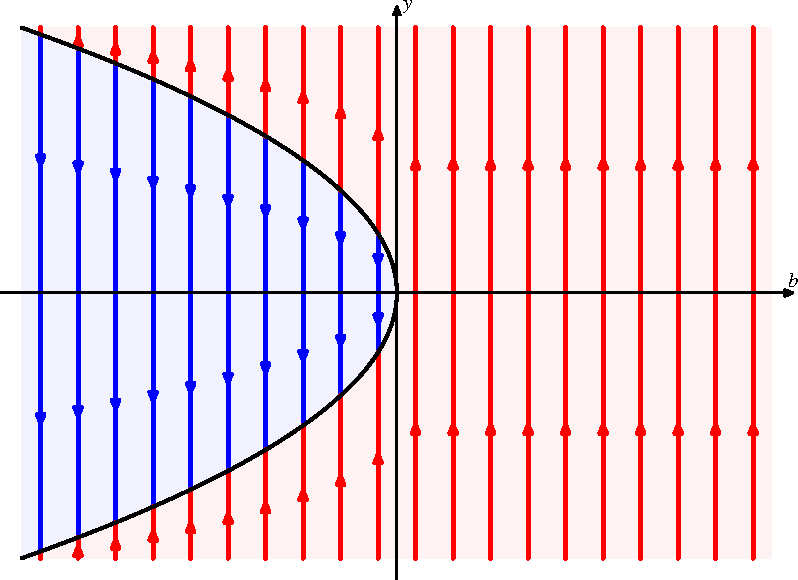
\includegraphics{chapters/images/bifurkation-1.pdf}
\caption{Phasendiagramm f"ur die Sattel-Knoten-Bifurkation in
Abh"angigkeit vom Parameter $b$.
\label{geometrie:saddle-node}}
\end{figure}

\subsubsection{Heugabel-Bifurkation}
\begin{figure}
\centering
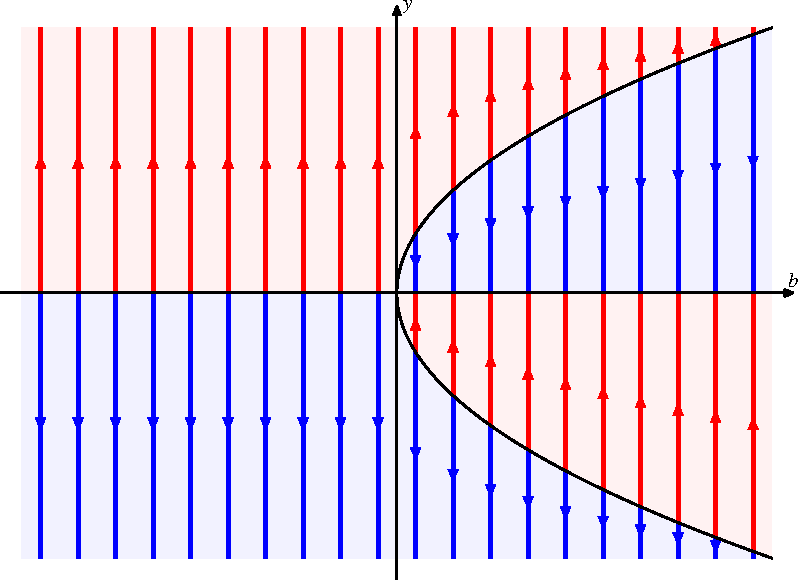
\includegraphics{chapters/images/bifurkation-2.pdf}
\caption{Phasendiagramm f"ur die Heugabel-Bifurkation in Abh"angigkeit vom
Parameter $b$.
\label{geometrie:pitchfork}}
\end{figure}
Eine andere Art von Bifurkatione zeigt das Modell
\[
f(y,b)=y^3-by.
\]
F"ur $b<0$ hat die Funktion $y\mapsto f(y,b)$ nur die eine
reelle Nullstelle $y=0$.
F"ur $b>0$ dagegen liegen die drei verschiedenen Nullstellen
$-\sqrt{b}$, $0$  und $\sqrt{b}$.
Das zugeh"orige Phasendiagramm ist in Abbildung~\ref{geometrie:pitchfork}
dargestellt, diese Art von Bifurkation heisst {\em Heugabel-}
oder {\em Pitchformk-Bifurkation}.
\index{Heugabel-Bifurkation}
\index{Pitchfork-Bifurkation}
Bei dieser Art von Bifurkation werden aus einer Nullstelle deren drei.
War die Nullstelle instabil (wie in Abbildung~\ref{geometrie:pitchfork}),
entstehen zwei neue instabile Nullstellen, die bisherige Nullstellen 
wird stabil.
War die eine Nullstelle stabil, entstehen zwei stabile Nullstellen, die
eine Nullstelle wird instabil.

\subsubsection{Transkritische Bifurkation}
\begin{figure}
\centering
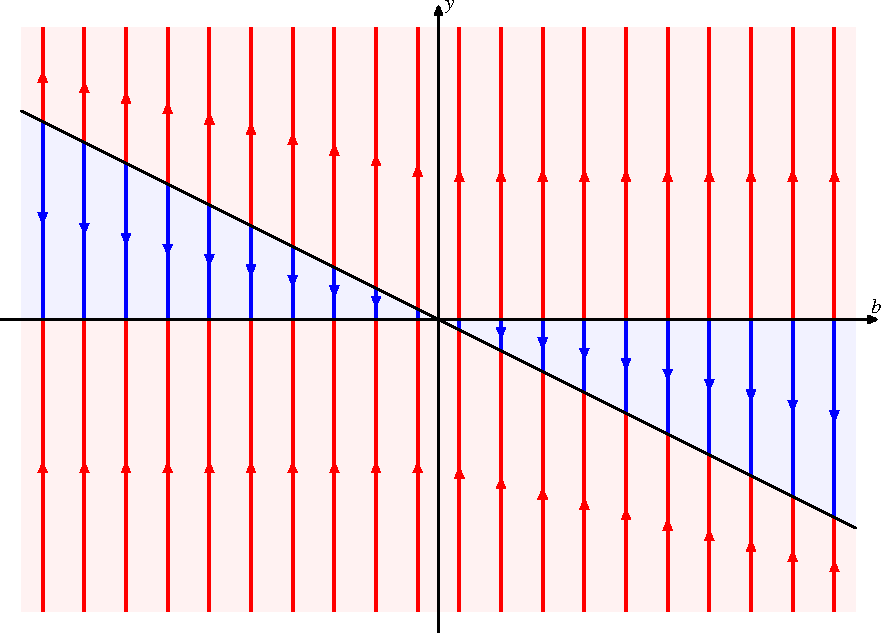
\includegraphics[width=\hsize]{chapters/images/bifurkation-3.pdf}
\caption{Phasendigramm f"ur die transkritische Bifurkation in Abh"angigkeit
vom Parameter $b$.
\label{geometrie:transkritisch}}
\end{figure}
Das Standard-Modell f"ur die sogenannten {\em transkritische Bifurkation} ist 
\index{transkritische Bifurkation}
\[
f(y,b)=y^2+yb = y(y+b)
\]
(Abbildung~\ref{geometrie:transkritisch}).
F"ur $b=0$ hat dieses System einen kritischen Punkt bei $y=0$.
Eine L"osungskurve, die bei negativem $y$ beginnt, wird immer n"aher
an den Punkt $y=0$ herankommen.
Liegt der Anfangswert jedoch im Gebiet $y>0$, wird sich die L"osungskurve
immer weiter von $y=0$ entfernen.
Der Fixpunkt bei $y=0$ ist also weder stabil noch instabil.

F"ur $b\ne 0$ entsteht ein weiterer kritischer Punkt bei $y=-b$.
Da f"ur $y\to\pm\infty$ die Funktion $y\mapsto f(y,b)$ immer positiv
ist, ist der rechte der beiden Fixpunkte immer stabil, der
linke immer instabil.


%
% Zweidimensionale Systeme
%
\section{Zweidimensionale Systeme}
In diesem Abschnitt betrachten wir die geometrischen Einschr"ankungen, denen
zweidimensionale autonome Systeme unterliegen.
Wieder sind Punkte von besonderem Interesse, in denen $f$ verschwindet.
Bei eindimensionalen Systemen teilen solche Punkte den $y$-Bereich in
verschiedene Intervall, in denen die Bewegung nur in jeweils
eine Richtung erfolgen kann, damit ist es leicht zu entscheiden,
ob ein solcher kritischer Punkt stabil oder instabil ist.
In zwei Dimensionen legen die Punkte alleine den Charakter noch nicht
fest, insbesondere ist es ja auch m"oglich, dass eine Bahn einen solche
Punkt umschliesst.

\subsection{Nullklinen}
Kritische Punkte von $f$ sind solche, in denen beide Komponenten
des Vektors $f(y)$ verschwinden.
Die Gleichungen
\[
f_1(y)=0
\qquad\text{und}\qquad
f_2(y)=0
\]
beschreiben zwei Kurvenscharen in der Ebene, die sogenannten 
{\em Nullklinen}.
\index{Nullkline}
Die Schnittpunkte von Nullklinen sind die kritischen Punkte.

Da auf einer Nullkline jeweils eine der Komponenten von $f(y)$ verschwindet,
schneiden L"osungskurven Nullklinen immer entweder horizontal oder
vertikal.
Ausserdem trennen die Nullklinen Gebiete unterschiedlicher Bewegungsrichtung
entlang einer Achse. 
Die Nullkline $f_1(y)=0$ trennt Gebiete, in denen sich eine L"osungskurve
nach rechts (zu gr"osseren $y_1$ hin) bewegt ($f_1(y)>0$) von Gebieten,
in denen sich die L"osungskurve nach links ($f_1(y)<0$) bewegt.
Desgleichen trennt die Nullkline $f_2(y)=0$ Gebiete mit Bewegung ``nach oben''
von Gebieten mit Bewegung ``nach unten''.
Allein aus dieser Information kann man sich bereits ein recht gutes
qualitives Bild "uber den Verlauf der L"osungen verschaffen, wie wir
im Folgenden an zwei Beispiel illustrieren wollen.

\begin{beispiel}
\begin{figure}
\centering
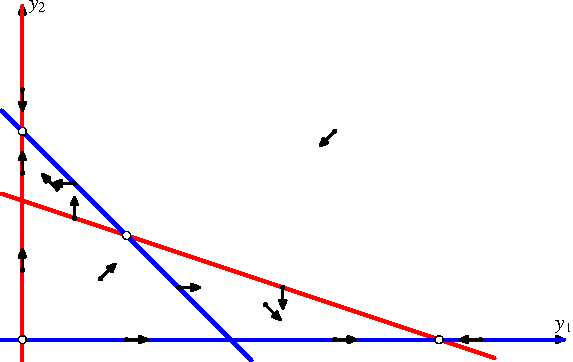
\includegraphics{chapters/images/nullklinen-1.pdf}
\caption{Nullklinen der Differentialgleichung~(\ref{geometrie:nullklinen-dgl1}),
die $y_1$-Nullklinen in rot, die $y_2$-Nullklinen in blau.
Kritische Punkte sind die Schnittpunkte verschiedenfarbiger Nullklinen.
\label{geometrie:nullklinen1}}
\end{figure}
Wir betrachten das nichtlineare System 
\begin{equation}
\frac{d}{dx} \begin{pmatrix}y_1\\y_2\end{pmatrix}
=
\begin{pmatrix}
2y_1\biggl(1-\displaystyle\frac{y_1}2\biggr)-3y_1y_2\\
y_2(1-y_2)-y_1y_2
\end{pmatrix}.
\label{geometrie:nullklinen-dgl1}
\end{equation}
Die direkte L"osung ist ziemlich aussichtslos, wir versuchen daher mit
Hilfe der Nullklinen ein qualitatives Bild
(Abbildung~\ref{geometrie:nullklinen1}) zu erhalten.

Die $y_2$-Nullkline hat die Gleichung
\[
0=y_2(1-y_2)-y_1y_2=y_2(1-y_2-y_1)
\qquad\Rightarrow\qquad
y_2=0
\quad\text{oder}\quad
y_1+y_2=1.
\]
L"osungskurven schneiden also die beiden Geraden $y_2=0$ (die $y_1$-Achse)
und $y_1+y_2=1$ horizontal.
Da die $y_1$-Achse bereits horizontal ist, bedeutet dies, dass sich die
L"osungskurven der $y_1$-Achse anschmiegen.

Die $y_1$-Nullkline hat die Gleichung
\[
0=2y_1\biggl(1-\frac{y_1}2\biggr)-3y_1y_2=y_1(2-y_1-3y_2),
\qquad\Rightarrow\qquad
y_1=0
\quad\text{oder}\quad
y_1+3y_2=2.
\]
Wir schliessen wieder, dass die L"osungskurven die $y_2$-Achse und
die Gerade $y_1+3y_2=3$ vertikal schneiden.
Da die $y_2$-Achse schon vertikal ist, m"ussen sich auch dort
die L"osungskurven anschmiegen.

Wir k"onnen aus den Nullklinen auch die kritischen Punkte ableiten.
Da sind zun"achst die Punkte auf den Achsen, also zum Beispiel
der Schnittpunkt der $y_2$-Nullkline $y_2=0$ mit der $y_1$-Nullkline
$y_1+3y_2=2$, also $(2,0)$, oder der Schnittpunkt der
$y_1$-Nullkline $y_1=0$ mit der $y_2$-Nullkline $y_1+y_2=0$, also $(0,1)$.
Ausserdem ist nat"urlich $(0,0)$ ein kritischer Punkt.
ein vierter kritischer Punkt entsteht als Schnittpunkt
der $y_1$-Nullkline $y_1+3y_2=2$ mit der $y_2$-Nullkline $y_1+y_2=1$,
also als L"osung des linearen Gleichungssystems
\[
\begin{linsys}{2}
y_1&+&3y_2&=&2\\
y_1&+& y_2&=1.
\end{linsys}
\]
Es hat die L"osung $(\frac23,\frac13)$, die kritischen Punkte sind also
\[
(0,0),\quad
(2,0),\quad
(0,1)\quad\text{und}\quad
\biggl(\frac23,\frac13\biggr).
\]

An den aus den Nullklinen l"asst sich auch die Bewegungsrichtung der
der L"osungen im Bezug auf die kritischen Punkte ablesen.
Aus dem Gebiet oben rechts und unten links in der N"ahe des Ursprungs
bewegen sich die L"osungen zun"achst auf den kritischen Punkt
bei $(\frac12,\frac12)$ zu, weichen dann aber ab in Richtung auf die
kritischen Punkte $(0,1)$ und $(2,0)$.
Die krtischen Punkte $(0,0)$ und $(\frac12,\frac12)$ sind also
instabil, w"ahrend $(2,0)$ und $(0,1)$ stabil sind.
Dies wird auch von dem genaueren Vektorfeld in
Abbildung~\ref{geometrie:nullklinen1} best"atigt.
\begin{figure}
\centering
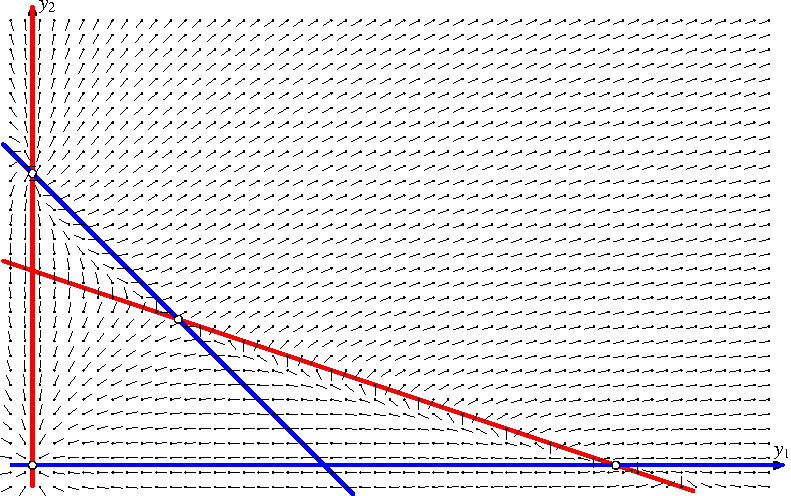
\includegraphics{chapters/images/nullklinen-2.pdf}
\caption{Vektorfeld der Differentialgleichung~(\ref{geometrie:nullklinen-dgl1}),
es best"atigt die Resultate der qualitiativen Diskussion aus
Abbildung~\ref{geometrie:nullklinen1}.
\label{geometrie:nullklinen-fluss}}
\end{figure}
\begin{figure}
\centering
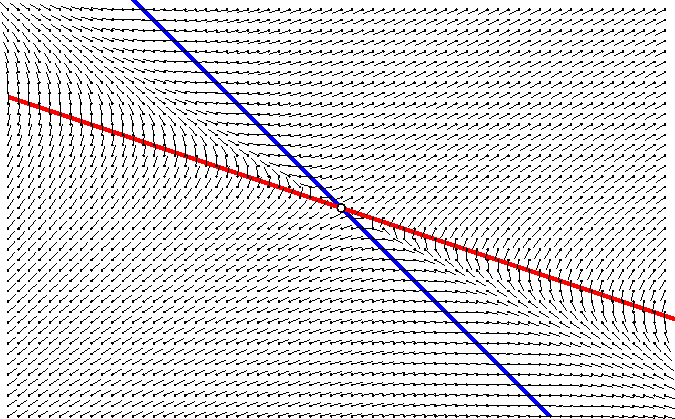
\includegraphics{chapters/images/nullklinen-3.pdf}
\caption{Vektorfeld der Differentialgleichung~(\ref{geometrie:nullklinen-dgl1})
in einer Umgebung des instabilen kritischen Punktes $(\frac12,\frac12)$.
\label{geometrie:nullklinen-instabil}}
\end{figure}
\begin{figure}
\centering
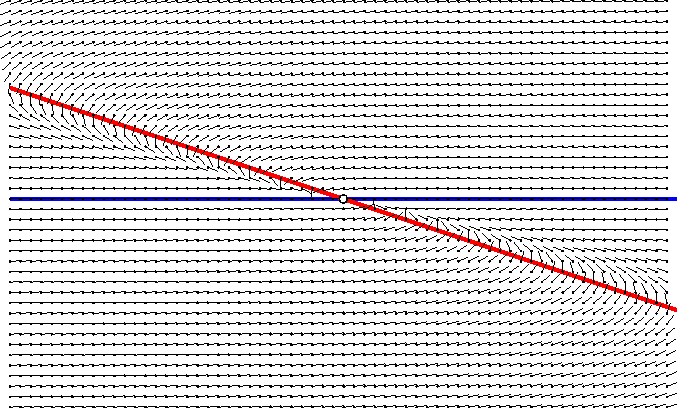
\includegraphics{chapters/images/nullklinen-4.pdf}
\caption{Vektorfeld der Differentialgleichung~(\ref{geometrie:nullklinen-dgl1})
in einer Umgebung des stabilen kritischen Punktes $(2,0)$.
\label{geometrie:nullklinen-stabil}}
\end{figure}
In Abschnitt~\label{geometrie:umgebung-kritisch} wird gezeigt, dass man 
die Bewegung in der Umgebung eines kritischen Punktes mit Hilfe der
Eigenwerte der Ableitungen klassifizieren kann.
Die Ableitungen, also die Jacobi-Matrix von $f$ ist
\[
\frac{\partial f}{\partial y}
=
\frac{\partial}{\partial y}
\begin{pmatrix}
2y_1-y_1^2-3y_1y_2\\
y_2-y_2^2-y_1y_2
\end{pmatrix}
=
\begin{pmatrix}
2-2y_1-3y_2 & -3y_1\\
-y_2        &1-2y_2-y_1
\end{pmatrix}
\]
In den vier kritischen Punkten finden wir die folgenden Matrizen und
Eigenwerte
\begin{align*}
&(0,0)
	&\frac{\partial f}{\partial y}&=\begin{pmatrix}2&0\\0&1\end{pmatrix}
		&&\lambda_1=2,\;\lambda_2=1\\
&(2,0)
	&\frac{\partial f}{\partial y}&=\begin{pmatrix}-2&-6\\0&-1\end{pmatrix}
		&&\lambda_1=-2,\;\lambda_2=-1\\
&(0,1)
	&\frac{\partial f}{\partial y}&=\begin{pmatrix}-1&0\\-1&-1\end{pmatrix}
		&&\lambda_1=-1,\;\lambda_2=-1\\
&\textstyle(\frac12,\frac12)
	&\frac{\partial f}{\partial y}&=\begin{pmatrix}-\frac12&-\frac32\\-\frac12&-\frac12\end{pmatrix}
		&&\lambda_1=\frac{\sqrt{3}-1}2,\;\lambda_2=-\frac{\sqrt{3}+1}2
\end{align*}
Nur bei den Punktein $(2,0)$ und $(0,1)$ sind beide Eigenwerte negativ,
nur diese beiden Punkte sind stabil, wie bereits die  Diskussion der
Nullklinen gezeigt hat.
\end{beispiel}

\begin{beispiel}
Das {\em Fitzhugh-Nagumo-Modell} wird verwendet, um das Verhalten eines Neurons
zu simulieren.
\index{Fitzhugh-Nagumo-Modell}
Es verwendet das Differentialgleichungssystem
\begin{align*}
    \dot v&= v-\frac13v^3-w\\
\tau\dot w&= v-a-bw.
\end{align*}
Wir versuchen uns wieder mit Hilfe der Nullklinen ein Bild von den
L"osungskurven zu verschaffen.
Die $v$-Nullkline hat die Gleichung
\[
0=v-\frac13v^3-w
\qquad\Rightarrow\qquad
w=v-\frac13v^3 = v(1-{\textstyle\frac1{\sqrt{3}}}v)(1+{\textstyle\frac1{\sqrt{3}}}v)
\]
Diese kubische Parabel hat im Nullpunkt die Steigung $1$.
Die $w$-Nullkline ist die Gerade
\[
0=v-a-bw
\qquad\Rightarrow\qquad
v=bw+a
\qquad\Rightarrow\qquad
w = \frac{v-a}{b}.
\]
Wenn die Steigung $1/b$ dieser Geraden gr"osser als $1$ ist, dann schneidet
die Gerade die kubische Parabel nur in einem Punkt, es gibt dann nur
einen kritischen Punkt.
Ist die Steigung $1/b<1$, gibt es f"ur nicht zu grosses $|a|$ drei
Schnittpunkte.

\begin{figure}
\centering
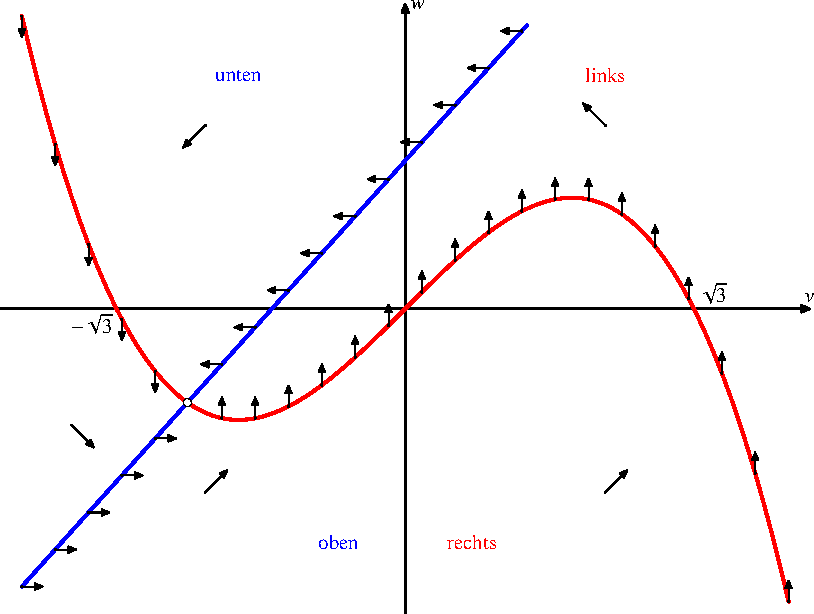
\includegraphics{chapters/images/nullklinen-5.pdf}
\caption{Nullklinen des Fitzhugh-Nagumo-Modells bei nur einem kritischen Punkt,
$a=-0.8$, $b=0.9$.
\label{geometrie:nullklinen-fh-1}}
\end{figure}
In Abbildung~\ref{geometrie:nullklinen-fh-1} sind die Nullklinen des
Fitzhugh-Nagumo-Modells dargestellt mit nur einem kritischen Punkt dargestellt.
Die L"osungskurven bewegen sich in Spiralen im Gegenurzeigersinn
um den Fixpunkt herum.
In diesem Fall erlauben die Nullklinen keine abschliessende Beurteilung
der Stabilit"at des Fixpunktes.

\begin{figure}
\centering
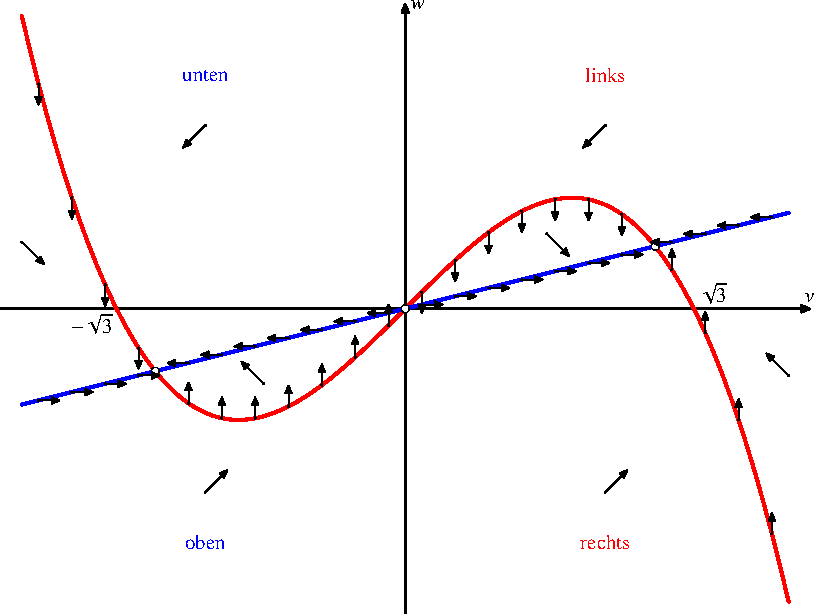
\includegraphics{chapters/images/nullklinen-6.pdf}
\caption{Nullklinen des Fitzhugh-Nagumo-Modells mit drei kritischen Punkten,
$b=4$, $a=0$.
\label{geometrie:nullklinen-fh-2}}
\end{figure}
In Abbildung~\ref{geometrie:nullklinen-fh-2} sind die Nullklinen des
Fitzhugh-Nagumo-Modells dargstellt mit drei kritschen Punkten.
Man kann sofort ablesen, dass $(0,0)$ ein instabiler kritischer Punkt ist.
Die L"osungskurven, die von diesem Punkt abgesteossen werden, n"ahern sich
einem der beiden anderen kritischen Punkte und bewegen sich
in einer Spirale um diesen Punkt herum.
Da sich die L"osungskurven nicht schneiden d"urfen kann man folgern,
dass die beiden anderen kritschen Punkte stabil sein m"ussen,
die L"osungskurven werden sich ihnen in Spiralbahnen n"ahern.
\end{beispiel}

%
% Bewegung in der Umgebung eines kritischen Punktes
%
\subsection{Bewegung in der Umgebung eines kritischen Punktes\label{geometrie:umgebung-kritisch}}
Wir gehen jetzt davon aus, dass 
\[
y'=f(y)
\]
einen kritischen Punkt hat, wir k"onnen die Koordinaten immer so w"ahlen,
dass der kritische Punkt im Nullpunkt des Koordinatensystems liegt.
Die Bewegung in unmittelbarer Umgebung des Nullpunktes kann dann approximiert
werden durch die Bewegung des linearisierten Systems
\[
y'=\frac{\partial f(0)}{\partial y}y
\]
Die m"oglichen Bewegungsformen in der Umgebung des kritischen Punktes
sind also bestimmt durch die Jacobi-Matrix.
Jede beliebige $2\times 2$-Matrix kann auch tats"achlich als Jacobi-Matrix
vorkommen, denn das System
$
y'=Ay
$
hat die Matrix $A$ als Jacobi-Matrix.

Wir interessieren uns im Moment nur f"ur eine qualitative Beschreibung
der L"osungen, wir k"onnen also immer eine Koordinatentransformation
vornehmen, um die Situation zu vereinfachen.
Die gesuchte qualitative Klassifizierung von zweidimensionalen
Differentialgleichungssystemen l"auft also auf eine Klassifizierung
von reellen $2\times 2$-Matrizen bis auf Koordinatentransformation
hinaus.

Eine solche Klassifikation kann auf der Basis von Eigenwerten und
Eigenvektoren erfolgen.
Dazu ben"otigen wir eine "Ubersicht "uber die Eigenwerte einer
Matrix
\[
A=\begin{pmatrix}a&b\\c&d\end{pmatrix},
\]
die wir als Nullstellen des charakteristischen Polynoms bestimmen
k"onnen.
Das charakteristische Polynom ist
\[
\chi_A(\lambda)
=
\det(A-\lambda E)
=
\left|\,\begin{matrix}a-\lambda&b\\c&d-\lambda\end{matrix}\,\right|
=
(a-\lambda)(d-\lambda)-bc
=
\lambda^2-(a+b)\lambda + ad-bc,
\]
es ist bestimmt durch die Spur und die Determinante der Matrix
\[
\begin{aligned}
\det A&=ad -bc,
&
\operatorname{Spur}A&=a+d
&
&\Rightarrow
&
\chi_A(\lambda)&=\lambda^2-\lambda \operatorname{Spur}A+\det A
\end{aligned}
\]
Die L"osungsformel f"ur die quadratische Gleichung liefert die
Eigenwerte
\[
\lambda_{1,2}
=
\frac{\operatorname{Spur}A}2\pm\sqrt{\Delta}
\qquad
\qquad
\text{mit}\quad
\Delta = \biggl(\frac{\operatorname{Spur}A}2\biggr)^2 - \det A
\]
Falls die Diskriminanten $\Delta > 0$ ist, sind die beiden Eigenwerte
verschieden, und folglich gibt es zwei verschiedene Eigenvektoren,
die Matrix $A$ kann diagonalisiert werden mit Diagonalelementen
$\lambda_{1,2}$.  Das Differentialgleichungssystem zerf"allt dann
in zwei unabh"angige eindimensionale Systeme
\begin{align*}
y_1'&= \lambda_1 y_1\\
y_2'&= \lambda_2 y_2,
\end{align*}
die auch durch
\begin{align*}
y_1(x)&=y_{10} e^{\lambda_1 x}\\
y_2(x)&=y_{20} e^{\lambda_2 x}
\end{align*}
sofort gel"ost werden k"onnen.
F"ur die Diskussion der Form der L"osungskurven brauchen wir aber die
Abh"angigkeit der beiden Koordinaten untereinander, nicht von $x$.
Wir stellen daher $y_2$ als Funktion von $y_1$ dar:
\[
y_1=y_{10} e^{\lambda_1 x}
\qquad\Rightarrow\qquad
x=\frac1{\lambda_1}\log\frac{y_1}{y_{10}}
\qquad\Rightarrow\qquad
y_2
=
y_{20} e^{\frac{\lambda_2}{\lambda_1}\log\frac{y_1}{y_{10}}}
=
y_{20}\biggl(\frac{y_1}{y_{10}}\biggr)^{\frac{\lambda_2}{\lambda_1}}
=
Cy^{\frac{\lambda_2}{\lambda_1}}
\]
\begin{figure}
\centering
\begin{tabular}{ccc}
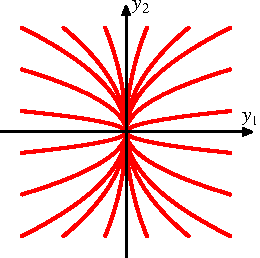
\includegraphics{chapters/images/geometrie-2.pdf}&%
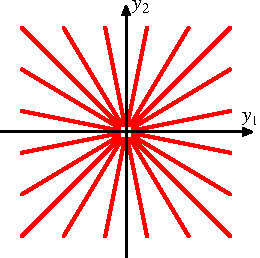
\includegraphics{chapters/images/geometrie-3.pdf}&%
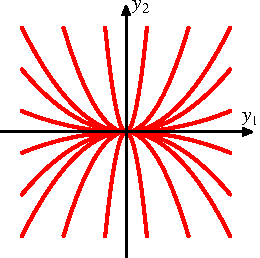
\includegraphics{chapters/images/geometrie-4.pdf}\\
$\displaystyle \frac{\lambda_2}{\lambda_1}>1$&%
$\displaystyle \frac{\lambda_2}{\lambda_1}=1$&%
$\displaystyle \frac{\lambda_2}{\lambda_1}<1$
\end{tabular}
\caption{L"osungskurven des linearisierten Systems f"ur
$\frac{\lambda_2}{\lambda_1}>0$.
\label{geometrie:posportraits}}
\end{figure}

\begin{figure}
\centering
\begin{tabular}{ccc}
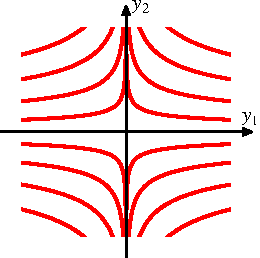
\includegraphics{chapters/images/geometrie-5.pdf}&%
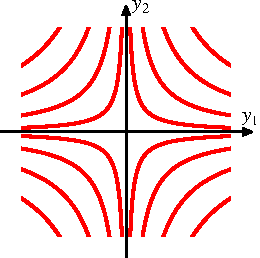
\includegraphics{chapters/images/geometrie-6.pdf}&%
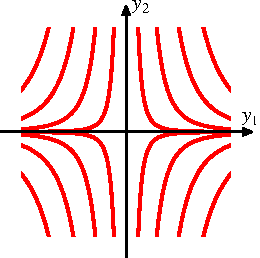
\includegraphics{chapters/images/geometrie-7.pdf}\\
$\displaystyle \frac{\lambda_2}{\lambda_1}>-1$&%
$\displaystyle \frac{\lambda_2}{\lambda_1}=-1$&%
$\displaystyle \frac{\lambda_2}{\lambda_1}<-1$
\end{tabular}
\caption{L"osungskurven des linearisierten Systems f"ur
$\frac{\lambda_2}{\lambda_1}<0$.
\label{geometrie:negportraits}}
\end{figure}
Die Gestalt der L"osungskurven sind also im Wesentlichen durch den
Quotienten $\lambda_2/\lambda_1$ bestimmt.
Die Abbildung~\ref{geometrie:posportraits} zeigt die L"osungskurven
f"ur positive Werte des Quotienten, w"ahrend
Abbildung~\ref{geometrie:negportraits} die L"osungskurven f"ur
negative Werte des Quotienten zeigt.
F"ur positive Werte von $\lambda_2/\lambda_1$ bewegen sich die 
Punkte entweder immer auf den kritischen Punkt zu, oder entfernen
sich.
F"ur negative Werte von $\lambda_2/\lambda_1$ n"ahert sich ein
Punkt in der N"ahe der einen Achse zun"achst immer mehr dem kritischen
Punkt, um sich dann in Richtung der anderen Achse zu entfernen.

Die Matrix $A$ muss jedoch nicht diagonalisierbar sein, wenn
$\lambda_1=\lambda_2$.
Wenn die Matrix nur einen Eigenvektor hat, dann kann die Matrix
durch eine geeignete Koordinatentransformation in die Form
\[
\begin{pmatrix}
\lambda&      1\\
      0&\lambda
\end{pmatrix}
\]
bringen.
Die Differentialgleichungen lauten in diese Fall
\begin{align*}
y_1'&=\lambda y_1 + y_2\\
y_2'&=\lambda y_2
\end{align*}
Die zweite Gleichung kann wie vorher gel"ost werden, die L"osung f"ur $y_2$
ist
\[
y_2(x)=y_{20}e^{\lambda x},
\]
dies k"onnen wir in die erste Gleichung einsetzen, sie lautet jetzt
\[
y_1' = \lambda y_1 + y_{20}e^{\lambda x},
\]
dies ist wieder eine lineare Differentialgleichung, diesmal jedoch
eine inhomogene. 
Die L"osung der homogenen Gleichung ist $Ce^{\lambda x}$, die L"osung
der inhomogenen Gleichung kann durch Variation der Konstanten gefunden
werden, also $y_1(x)=C(x)e^{\lambda x}$.
Setzen wir dies in die Differentialgleichung 
\[
y_1'(x)
=
C'(x)e^{\lambda x}+C(x)\lambda e^{\lambda x}
=
\lambda y_1(x) + C'(x)e^{\lambda x}
=
\lambda y_1(x) + y_{20}e^{\lambda x}
\]
ein.
Diese Gleichung kann nur erf"ullt sein, wenn
\[
C'(x)=y_{20}
\qquad\Rightarrow\qquad
C(x)=y_{20}x+y_{10},
\]
die L"osung der Gleichung ist also
\[
y(x)=\begin{pmatrix}
y_{20}x+y_{10}\\
y_{20}
\end{pmatrix}e^{\lambda x}.
\]
\begin{figure}
\centering
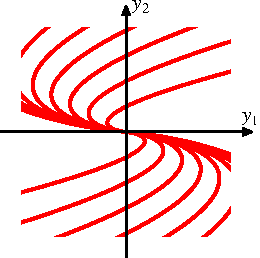
\includegraphics{chapters/images/geometrie-8.pdf}
\caption{L"osungskurven f"ur den Fall nicht diagonalisierbarer Jacobi-Matrix
mit zwei gleichen Eigenwerten.
\label{geometrie:jnf-kurven}}
\end{figure}%
In Abbildung~\ref{geometrie:jnf-kurven} sind die L"osungskurven dargestellt.
F"ur $\lambda >0$ streben die L"osungskurven gegen den Nullpunkt, aber auf
eine Art, sie im Grenzfall die $y_1$-Achse ber"uhren.

Falls die Diskriminante $\Delta$ negativ ist, gibt es keine reellen
Eigenwerte, also auch keine reellen Eigenvektoren.
Wir k"onnen aber trotzdem eine Basis finden, in der die Geometrie
dar Bahnkurven leichter verst"andlich ist.
Dazu schreiben wir 
\[
\alpha = \frac{\operatorname{Spur}A}2=\frac{a+d}2
\qquad
\text{und}
\qquad
\beta = \sqrt{-\Delta},
\]
und betrachten die beiden Vektoren
\[
w_1 = \begin{pmatrix}0\\\beta\end{pmatrix}.
\qquad\text{und}\qquad
w_2 = \begin{pmatrix}b\\\alpha-a\end{pmatrix}
\]
Wir berechnen die Wirkung der Matrix $A$ auf diesen beiden Vektoren,
und zerlegen jeweils das Resultat wieder in $w_1$ und $w_2$:
\begin{align*}
Aw_1
&=
\begin{pmatrix}a&b\\c&d\end{pmatrix}
\begin{pmatrix}0\\\beta\end{pmatrix}
=
\begin{pmatrix}
\beta b\\
\beta d
\end{pmatrix}
=
v
\begin{pmatrix}0\\\beta\end{pmatrix}
+
\beta
\begin{pmatrix}b\\\alpha-a\end{pmatrix}
\\
Aw_2
&=
\begin{pmatrix}a&b\\c&d\end{pmatrix}
\begin{pmatrix}b\\\alpha-a\end{pmatrix}
=
\begin{pmatrix}
ab-ab+b\alpha\\
bc-ad+\alpha d
\end{pmatrix}
=
\alpha
\begin{pmatrix}b\\\alpha-a\end{pmatrix}
+u
\begin{pmatrix}0\\\beta\end{pmatrix}
\end{align*}
Wir m"ussen nur noch die Konstanten $u$ und $v$ bestimmen:
\begin{align*}
\beta d
&=
v\beta
+
\alpha\beta
-
\beta a
&&\Rightarrow&
v
&=
\alpha a+d-\alpha=2\alpha-\alpha=\alpha
\\
-\det A +\alpha d
&=
\alpha^2- \alpha a+u\beta
&&\Rightarrow&
u\beta&=-\det A +\alpha(a+d)-\alpha^2
=\alpha^2-\det A
=\Delta=-\beta^2
\end{align*}
Aus der zweiten Gleichung folgt $ u=-\beta$.
Damit haben wir die Wirkung der Matrix $A$ auf den Vektoren $w_1$ und $w_2$
bestimmt, und wir k"onnen daraus die Matrix von $A$ in der Basis
$\{w_1,w_2\}$ ablesen, wir bezeichnen sie mit $A'$
\[
\begin{aligned}
Aw_1&=\alpha w_1 + \beta w_2\\
Aw_2&=-\beta w_1 + \alpha w_2
\end{aligned}
\qquad\Rightarrow\qquad
A'=\begin{pmatrix}
\alpha&\beta\\
-\beta&\alpha
\end{pmatrix}
\]
Dies ist die gesuchte Form der Matrix, in der sich die L"osungskurven
leichter beschreiben lassen.
Eine L"osung daf"ur l"asst sich angeben, wenn man ber"ucksichtigt, dass
$A'$ einer Drehmatrix "ahnelt.
Wir vermuten daher, dass die L"osungskurve im wesentlichen den kritischen
Punkt umkreist, m"oglicherweise mit einer "Anderung des Abstandes
zum kritischen Punkt, und schreiben daher
\begin{equation}
y(x)
=
\begin{pmatrix}
r_0e^{ux}\cos(vx+\delta_0)\\
r_0e^{ux}\sin(vx+\delta_0)
\end{pmatrix}
=
r_0e^{ux}
\begin{pmatrix}
\cos(vx+\delta_0)\\
\sin(vx+\delta_0)
\end{pmatrix}
,
\label{geometrie:rotsol}
\end{equation}
wobei wird $r_0$ und $\delta_0$ so w"ahlen, dass
\[
y_{10}=r_0\cos\delta_0
\qquad\text{und}\qquad
y_{20}=r_0\sin\delta_0.
\]
Setzen wir jetzt den Ansatz~(\ref{geometrie:rotsol}) in die
Differentialgleichung ein, erhalten wir
\begin{align*}
y'(x)
&=
\begin{pmatrix}
r_0ue^{ux}\cos(vx+\delta_0)-r_0e^{ux}v\sin(vx+\delta_0)\\
r_0ue^{ux}\sin(vx+\delta_0)+r_0e^{ux}v\cos(vx+\delta_0)
\end{pmatrix}
\\
&=
\begin{pmatrix}
 \alpha&\beta\\
-\beta &\alpha
\end{pmatrix}
\begin{pmatrix}
r_0e^{ux}\cos(vx+\delta_0)\\
r_0e^{ux}\sin(vx+\delta_0)
\end{pmatrix}
=
\begin{pmatrix}
r_0e^{ux}\alpha\cos(vx+\delta_0)+r_0e^{ux}\beta\sin(vx +\delta_0)\\
-r_0e^{ux}\beta\cos(vx+\delta_0)+r_0e^{ux}\alpha\sin(vx+\delta_0)
\end{pmatrix}
\end{align*}
Diese Gleichung ist genau dann korrekt, wenn 
\[
u=\alpha
\qquad\text{und}\qquad
v=-\beta.
\]
Die Zahlen $\alpha$ und $\beta$ charakterisieren also wieder die L"osung.
F"ur $\alpha < 0$ n"ahern sich die L"osungen dem kritischen Punkt, f"ur
$\alpha>0$ entfernen sie sich.
Die Zahl $\beta$ ist die Winkelgeschwindigkeit, mit der die L"osung
um den kritischen Punkt rotiert.
Die L"osungskurven sind daher Spiralen um den kritischen Punkt, sie
sind in Abbildung~\ref{geometrie:rotkurv} dargestellt.
\begin{figure}
\centering
\begin{tabular}{ccc}
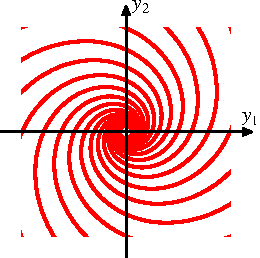
\includegraphics{chapters/images/geometrie-9.pdf}&%
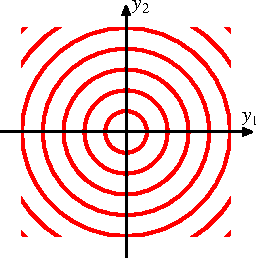
\includegraphics{chapters/images/geometrie-11.pdf}&%
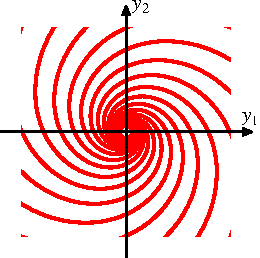
\includegraphics{chapters/images/geometrie-10.pdf}\\
$\alpha > 0$&$\alpha = 0$&$\alpha < 0$
\end{tabular}
\caption{L"osungskurven des linearisierten Systems im Falle $\Delta < 0$
sind Spiralen um den kritischen Punkt
\label{geometrie:rotkurv}}
\end{figure}

%
% Komplexe Eigenwerte
%
\subsection{Komplexe Eigenwerte}
Die Darstellung im vorangegangenen Abschnitt war darum bem"uht,
komplexe Zahlen zu vermeiden.
Die Darstellung im Falle $\Delta<0$ wurde dadurch unn"otig verkompliziert,
in diesem Abschnitt soll gezeigt werden, wie die Formeln f"ur die Vektoren
$w_1$ und $w_2$ mit Hilfe komplexer Zahlen hergeleitet werden k"onnen.

Zun"achst halten wir fest, dass im Falle $\Delta<0$ zwei konjugiert
komplexe Eigenwerte
$
\lambda= \alpha + i\beta
$
und
$
\overline{\lambda}= \alpha - i\beta
$
existieren.
Nehmen wir an, dass $v$ ein Eigenvektor zum Eigenwert $\lambda$ ist,
dann ist $\overline{v}$, dessen Komponenten die konjugiert komplexen
Komponenten von $v$ sind, ein Eigenvektor zum Eigenwert $\overline{\lambda}$.
Grund daf"ur ist die Tatsache, dass die Matrix $A$ nur reelle Matrixelemente
hat, also gilt
\[
A\overline{v}
=
\overline{Av}
=
\overline{\lambda v}=\overline{\lambda}\overline{v}.
\]
Der Vektor $v$ ist nat"urlich nicht geeignet f"ur eine reelle Beschreibung
der L"osungskurven des linearisierten Systems.
Wir konstruieren daher die Vektoren
\begin{equation}
\begin{aligned}
w_1&=\frac{i}2(v-\overline v)
&&\qquad
&
v&=-iw_1+w_2
\\
w_2&=\frac12(v+\overline v)
&&\qquad
&
\overline{v}&=iw_1+w_2
\end{aligned}
\label{geometrie:wv}
\end{equation}
und untersuchen, wie die Matrix $A$ darauf wirkt:
\begin{align*}
Aw_1
&=
\frac{i}2(Av-A\overline v)
=
\frac{i}2(\lambda v-\overline{\lambda}\overline{v})
\\
Aw_2
&=
\frac12(Av+A\overline{v})
=
\frac12(\lambda v+\overline{\lambda}\overline{v}).
\end{align*}
Setzen wir die Darstellungen von $v$ und $\overline{v}$ durch $w_i$ aus 
(\ref{geometrie:wv}) ein, und erhalten:
\begin{align*}
\frac{i}2(\lambda v-\overline{\lambda}\overline{v})
&=
\frac{i}2(\lambda(-iw_1+w_2) -\overline{\lambda}(iw_1+w_2))
=
\frac{1}2(\lambda+\overline{\lambda}) w_1
+
\frac{i}2(\lambda-\overline{\lambda}) w_2
=\alpha w_1-\beta w_2
\\
\frac12(\lambda v+\overline{\lambda}\overline{v})
&=
\frac12(\lambda(-iw_1+w_2)+\overline{\lambda}(iw_1+w_2))
=
-\frac{i}2(\lambda-\overline{\lambda}) w_1
+
\frac12(\lambda+\overline{\lambda}) w_2.
=\beta w_1+\alpha w_2
\end{align*}
Verwendet man also $\{w_1,w_2\}$ als Basis, dann bekommt die Matrix die
Form
\begin{equation}
A'=\begin{pmatrix}
\alpha&-\beta\\
\beta &\alpha
\end{pmatrix}
\label{geometrie:drehmatrix}
\end{equation}
Auf Grund der Konstruktion haben die Vektoren $w_1$ und $w_2$ reelle
Komponenten, $w_1$ ist der Realteil des Vektors $v$, $w_2$ ist
der Imagin"arteil.
Damit haben wir ein Rezept, wie wir eine Basis von reellen Vektoren
konstruieren k"onnen, in denen das System die
Form~(\ref{geometrie:drehmatrix}) hat.

Die Komponenten eines Eigenvektors $v$ erf"ullen die Gleichung
\[
(a-\lambda)v_1 + bv_2=0
\]
eine L"osung daf"ur ist
\[
v=\begin{pmatrix}
-b\\
a-\alpha-i\beta
\end{pmatrix},
\]
dessen Real- und Imagin"arteile
\[
\begin{pmatrix}
-b\\a-\alpha
\end{pmatrix}
\qquad\text{und}\qquad
\begin{pmatrix}
0\\\beta
\end{pmatrix},
\]
dies sind die Vektoren, die im vorangegangenen Abschnitt aus dem "Armel
gesch"uttelt worden waren, um die Matrix des Systems in die
Form~(\ref{geometrie:drehmatrix}) zu bringen.

%
% Hopf-Bifurkation
%
\subsection{Hopf-Bifurkation}
\begin{figure}
\centering
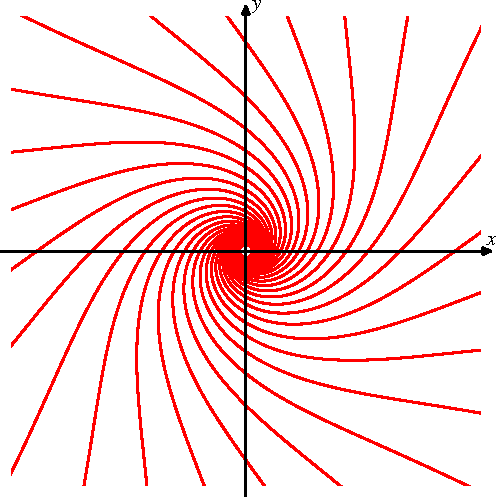
\includegraphics{chapters/images/hopf-1.pdf}
\caption{Fluss f"ur $b<0$, der kritische Punkt ist stabil,
Bahnkurven konvergieren gegen $0$.
\label{geometrie:hopf1}}
\end{figure}%
\begin{figure}
\centering
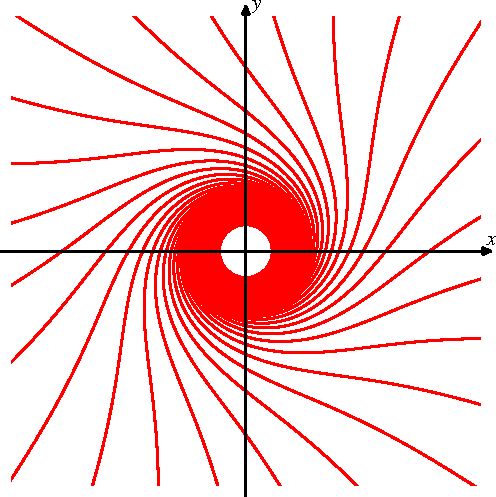
\includegraphics{chapters/images/hopf-2.pdf}
\caption{Fluss f"ur $b=0$, der kritische Punkt ist immer noch stabil,
die Bahnkurven n"ahern sich jedoch nicht mehr exponentiell schnell
dem Nullpunkt.
\label{geometrie:hopf2}}
\end{figure}%
\begin{figure}
\centering
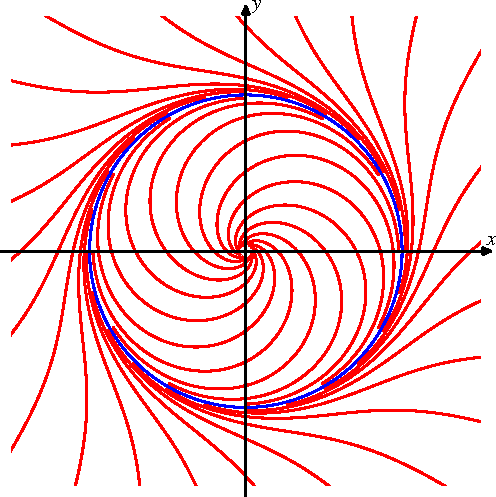
\includegraphics{chapters/images/hopf-3.pdf}
\caption{Fluss f"ur $b>0$, der Nullpunkt ist nicht mehr stabil, daf"ur
ist der Kreis mit Radius $\sqrt{b}$ eine stabile periodische Bahn (blau),
gegen die alle Bahnkurven exponentiell schnell konvergieren.
\label{geometrie:hopf3}}
\end{figure}%
\begin{figure}
\centering
\begin{tabular}{ccc}
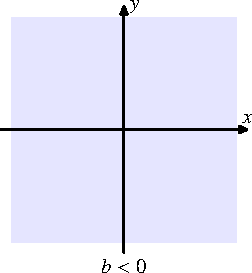
\includegraphics{chapters/images/hopf-4.pdf}&%
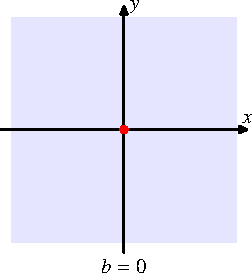
\includegraphics{chapters/images/hopf-5.pdf}&%
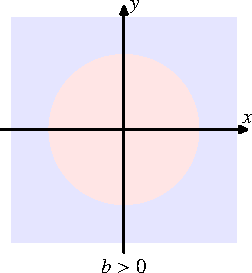
\includegraphics{chapters/images/hopf-6.pdf}%
\end{tabular}
\caption{Vorzeichen von $\dot r$ in Abh"angigkeit von $b$.
Punkte mit $\dot r <0$ sind blau gef"arbt, Punkte mit $\dot r >0$ rot.
\label{geometrie:hopfvorzeichen}}
\end{figure}%
Die in Abschnitt~\ref{geometrie:subsection:bifurkationen} untersuchten
Bifurkationen eindimensionaler Differentialgleichungen k"onnen in
analoger Form auch bei zweidimensionalen Differentialgleichungen auftreten.
Sie sind jedoch immer eindimensionale Bifurkationen, die entlang der
durch die Eigenvektoren der Linearisierung gegebenen Richtungen
auftreten.

Die h"ohere Dimensionszahl erlaubt aber auch eine Bifurkation, bei der
ein stabiler Fixpunkt in stabil wird und einen stabilen Zyklus ``abwirft''
(Abbildungen~\ref{geometrie:hopf1}, \ref{geometrie:hopf2} and
\ref{geometrie:hopf3}).
Wir betrachten dazu das System 
\begin{equation}
\begin{aligned}
\dot r      &= r(b-r^2)\\
\dot \varphi&= -1
\end{aligned}
\label{geometrie:hopfsystem}
\end{equation}
in Polarkoordinaten.
Offenbar ist $r=0$ ein Fixpunkt.
F"ur $b>0$ gibt es ausserdem eine periodische Bahn mit $r=\sqrt{b}$
(Abbildung~\ref{geometrie:hopf3}).
Wir wollen die Stabilit"at des Fixpunktes sowie der periodischen Bahn
untersuchen.
Die Abbildung~\ref{geometrie:hopfvorzeichen} fasst die f"ur das Bahnverhalten
entscheidenden Vorzeichen in den drei F"allen $b<0$, $b=0$ und $b>0$
zusammen.

In Polarkoordinaten beschreibt die Gleichung f"ur $r$ eine
Heugabel-Bifurkation.
Der kritische Punkt $r$ ist f"ur $b<0$ stabil, er wird f"ur $b>0$
instabil, daf"ur entstehen zwei neue stabile kritische Punkte
$r=\pm\sqrt{b}$.

Unsere bisherige Theorie zur Beurteilung von Fixpunkten ging von
kartesischen Koordinaten aus, wir f"uhren daher die Analyse auch noch
in kartesischen Koordinaten durch.
Mit Hilfe von 
\[
\begin{aligned}
x&=r\cos\varphi&\dot x&=\dot r\cos\varphi-r\sin\varphi\cdot\dot\varphi\\
y&=r\sin\varphi&\dot y&=\dot r\sin\varphi+r\cos\varphi\cdot\dot\varphi
\end{aligned}
\]
kann das System~(\ref{geometrie:hopfsystem}) in kartesische Koordinaten
umgerechnet werden:
\begin{equation}
\begin{aligned}
\dot x&=r(b-r^2)\frac{x}{r}+y=(b-x^2-y^2)x+y\\
\dot y&=r(b-r^2)\frac{y}{r}-x=(b-x^2-y^2)y-x.
\end{aligned}
\label{geometrie:hopf-kartesisch}
\end{equation}
Zur Beurteilung der Stabilit"at des Nullpunktes berechnen wir die
Jacobi-Matrix
\[
J(x,y)=
\begin{pmatrix}
b-3x^2-y^2&1-2xy\\
-1-2xy&b-x^2-3y^2
\end{pmatrix}
\quad\Rightarrow\quad
J(0,0)=\begin{pmatrix}
b&1\\-1&b
\end{pmatrix}.
\]
Die Matrix $J(0,0)$ hat das charakteristische Polynom
\[
(b-\lambda)^2+1=0
\]
mit den Nullstellen
\[
\lambda=b\mp i.
\]
Stabilit"at wird durch das Vorzeichen des Realteils der Eigenwerte
bestimmt, wir lesen daher ab, dass der kritische Punkt $0$ stabil
ist f"ur $b<0$ und instabil f"ur $b>0$.

\section{"Ubungsaufgaben}
\begin{uebungsaufgaben}
\item
\input uebungsaufgaben/601.tex
\end{uebungsaufgaben}
